\documentclass{standalone}
\usepackage{tikz}
\usetikzlibrary{patterns, positioning}

\begin{document}
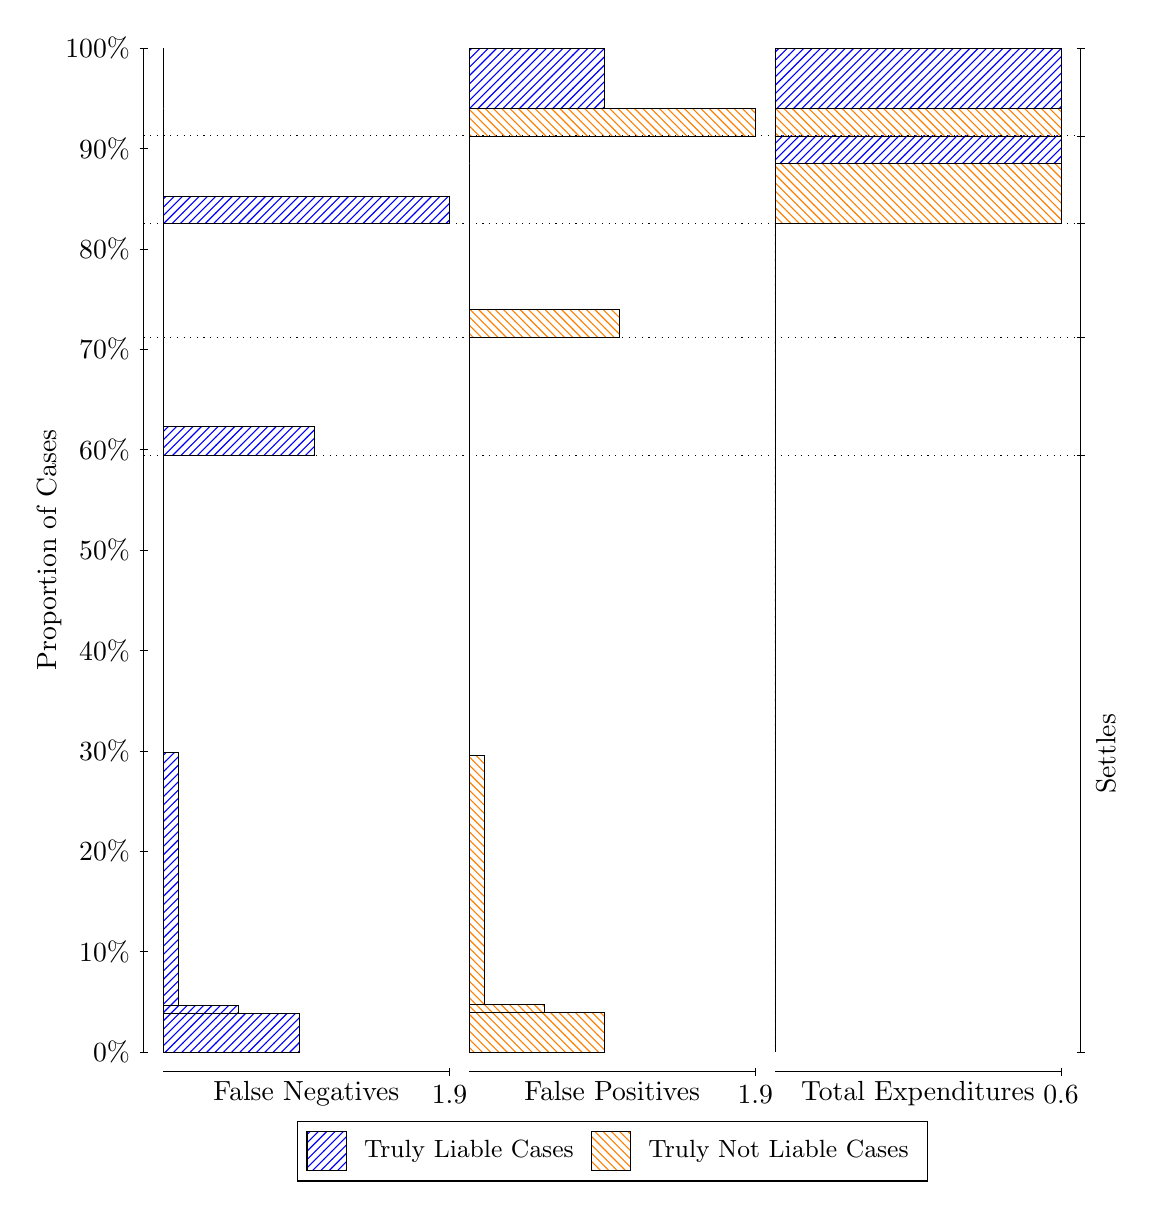
\begin{tikzpicture}
\draw[black, very thin] (1.5,1.75) -- (1.5,14.5);
\node[rotate=90, anchor=center] at (0.3, 8.125) {Proportion of Cases};
\draw[black, very thin] (1.45,1.75) -- (1.55,1.75);
\node[anchor=east] at (1.45, 1.75) {0\%};
\draw[black, very thin] (1.45,3.025) -- (1.55,3.025);
\node[anchor=east] at (1.45, 3.025) {10\%};
\draw[black, very thin] (1.45,4.3) -- (1.55,4.3);
\node[anchor=east] at (1.45, 4.3) {20\%};
\draw[black, very thin] (1.45,5.575) -- (1.55,5.575);
\node[anchor=east] at (1.45, 5.575) {30\%};
\draw[black, very thin] (1.45,6.85) -- (1.55,6.85);
\node[anchor=east] at (1.45, 6.85) {40\%};
\draw[black, very thin] (1.45,8.125) -- (1.55,8.125);
\node[anchor=east] at (1.45, 8.125) {50\%};
\draw[black, very thin] (1.45,9.4) -- (1.55,9.4);
\node[anchor=east] at (1.45, 9.4) {60\%};
\draw[black, very thin] (1.45,10.675) -- (1.55,10.675);
\node[anchor=east] at (1.45, 10.675) {70\%};
\draw[black, very thin] (1.45,11.95) -- (1.55,11.95);
\node[anchor=east] at (1.45, 11.95) {80\%};
\draw[black, very thin] (1.45,13.225) -- (1.55,13.225);
\node[anchor=east] at (1.45, 13.225) {90\%};
\draw[black, very thin] (1.45,14.5) -- (1.55,14.5);
\node[anchor=east] at (1.45, 14.5) {100\%};

\draw[black, very thin] (13.4,1.75) -- (13.4,14.5);
\draw[black, very thin] (13.35,1.75) -- (13.45,1.75);
\node[anchor=west] at (13.35, 1.75) {};
\draw[black, very thin] (13.35,9.3223) -- (13.45,9.3223);
\node[anchor=west] at (13.35, 9.3223) {};
\draw[black, very thin] (13.35,10.821) -- (13.45,10.821);
\node[anchor=west] at (13.35, 10.821) {};
\draw[black, very thin] (13.35,12.271) -- (13.45,12.271);
\node[anchor=west] at (13.35, 12.271) {};
\draw[black, very thin] (13.35,13.384) -- (13.45,13.384);
\node[anchor=west] at (13.35, 13.384) {};
\draw[black, very thin] (13.35,14.5) -- (13.45,14.5);
\node[anchor=west] at (13.35, 14.5) {};

\draw[black, very thin, pattern color=blue, pattern=north east lines] (1.75,1.75) rectangle (3.4711,2.2385);
\draw[black, very thin, pattern color=blue, pattern=north east lines] (1.75,2.2385) rectangle (3.2798,2.2389);
\draw[black, very thin, pattern color=blue, pattern=north east lines] (1.75,2.2389) rectangle (3.0886,2.2393);
\draw[black, very thin, pattern color=blue, pattern=north east lines] (1.75,2.2393) rectangle (2.8974,2.2397);
\draw[black, very thin, pattern color=blue, pattern=north east lines] (1.75,2.2397) rectangle (2.8974,2.2397);
\draw[black, very thin, pattern color=blue, pattern=north east lines] (1.75,2.2397) rectangle (2.7061,2.3434);
\draw[black, very thin, pattern color=blue, pattern=north east lines] (1.75,2.3434) rectangle (2.5149,2.3439);
\draw[black, very thin, pattern color=blue, pattern=north east lines] (1.75,2.3439) rectangle (2.3237,2.3444);
\draw[black, very thin, pattern color=blue, pattern=north east lines] (1.75,2.3444) rectangle (2.1325,2.3449);
\draw[black, very thin, pattern color=blue, pattern=north east lines] (1.75,2.3449) rectangle (1.9412,5.5515);
\draw[black, very thin, pattern color=orange, pattern=north west lines] (1.75,5.5515) rectangle (1.75,9.3223);
\draw[black, very thin, pattern color=blue, pattern=north east lines] (1.75,9.3223) rectangle (3.6623,9.6937);
\draw[black, very thin, pattern color=orange, pattern=north west lines] (1.75,9.6937) rectangle (1.75,10.821);
\draw[black, very thin, pattern color=orange, pattern=north west lines] (1.75,10.821) rectangle (1.75,11.185);
\draw[black, very thin, pattern color=blue, pattern=north east lines] (1.75,11.185) rectangle (1.75,12.271);
\draw[black, very thin, pattern color=blue, pattern=north east lines] (1.75,12.271) rectangle (5.3833,12.62);
\draw[black, very thin, pattern color=orange, pattern=north west lines] (1.75,12.62) rectangle (1.75,13.384);
\draw[black, very thin, pattern color=orange, pattern=north west lines] (1.75,13.384) rectangle (1.75,13.733);
\draw[black, very thin, pattern color=blue, pattern=north east lines] (1.75,13.733) rectangle (1.75,14.5);
\draw[black, very thin, pattern color=orange, pattern=north west lines] (5.6333,1.75) rectangle (7.3544,2.2508);
\draw[black, very thin, pattern color=orange, pattern=north west lines] (5.6333,2.2508) rectangle (7.1632,2.2511);
\draw[black, very thin, pattern color=orange, pattern=north west lines] (5.6333,2.2511) rectangle (6.9719,2.2515);
\draw[black, very thin, pattern color=orange, pattern=north west lines] (5.6333,2.2515) rectangle (6.7807,2.2519);
\draw[black, very thin, pattern color=orange, pattern=north west lines] (5.6333,2.2519) rectangle (6.5895,2.3563);
\draw[black, very thin, pattern color=orange, pattern=north west lines] (5.6333,2.3563) rectangle (6.3982,2.3563);
\draw[black, very thin, pattern color=orange, pattern=north west lines] (5.6333,2.3563) rectangle (6.3982,2.3568);
\draw[black, very thin, pattern color=orange, pattern=north west lines] (5.6333,2.3568) rectangle (6.207,2.3574);
\draw[black, very thin, pattern color=orange, pattern=north west lines] (5.6333,2.3574) rectangle (6.0158,2.3579);
\draw[black, very thin, pattern color=orange, pattern=north west lines] (5.6333,2.3579) rectangle (5.8246,5.5208);
\draw[black, very thin, pattern color=blue, pattern=north east lines] (5.6333,5.5208) rectangle (5.6333,9.3223);
\draw[black, very thin, pattern color=orange, pattern=north west lines] (5.6333,9.3223) rectangle (5.6333,10.45);
\draw[black, very thin, pattern color=blue, pattern=north east lines] (5.6333,10.45) rectangle (5.6333,10.821);
\draw[black, very thin, pattern color=orange, pattern=north west lines] (5.6333,10.821) rectangle (7.5456,11.185);
\draw[black, very thin, pattern color=blue, pattern=north east lines] (5.6333,11.185) rectangle (5.6333,12.271);
\draw[black, very thin, pattern color=orange, pattern=north west lines] (5.6333,12.271) rectangle (5.6333,13.036);
\draw[black, very thin, pattern color=blue, pattern=north east lines] (5.6333,13.036) rectangle (5.6333,13.384);
\draw[black, very thin, pattern color=orange, pattern=north west lines] (5.6333,13.384) rectangle (9.2667,13.733);
\draw[black, very thin, pattern color=blue, pattern=north east lines] (5.6333,13.733) rectangle (7.3544,14.5);
\draw[black, very thin, pattern color=orange, pattern=north west lines] (9.5167,1.75) rectangle (9.5167,5.5208);
\draw[black, very thin, pattern color=blue, pattern=north east lines] (9.5167,5.5208) rectangle (9.5167,9.3223);
\draw[black, very thin, pattern color=orange, pattern=north west lines] (9.5167,9.3223) rectangle (9.5167,10.45);
\draw[black, very thin, pattern color=blue, pattern=north east lines] (9.5167,10.45) rectangle (9.5167,10.821);
\draw[black, very thin, pattern color=orange, pattern=north west lines] (9.5167,10.821) rectangle (9.5167,11.185);
\draw[black, very thin, pattern color=blue, pattern=north east lines] (9.5167,11.185) rectangle (9.5167,12.271);
\draw[black, very thin, pattern color=orange, pattern=north west lines] (9.5167,12.271) rectangle (13.15,13.036);
\draw[black, very thin, pattern color=blue, pattern=north east lines] (9.5167,13.036) rectangle (13.15,13.384);
\draw[black, very thin, pattern color=orange, pattern=north west lines] (9.5167,13.384) rectangle (13.15,13.733);
\draw[black, very thin, pattern color=blue, pattern=north east lines] (9.5167,13.733) rectangle (13.15,14.5);
\draw[black, dotted] (1.5,9.3223) -- (13.4,9.3223);
\draw[black, dotted] (1.5,10.821) -- (13.4,10.821);
\draw[black, dotted] (1.5,12.271) -- (13.4,12.271);
\draw[black, dotted] (1.5,13.384) -- (13.4,13.384);
\draw[black, very thin] (1.75,1.5) -- (5.3833,1.5);
\node[anchor=north] at (3.5667, 1.5) {False Negatives};
\draw[black, very thin] (5.3833,1.45) -- (5.3833,1.55);
\node[anchor=north] at (5.3833, 1.45) {1.9};

\draw[black, very thin] (5.6333,1.5) -- (9.2667,1.5);
\node[anchor=north] at (7.45, 1.5) {False Positives};
\draw[black, very thin] (9.2667,1.45) -- (9.2667,1.55);
\node[anchor=north] at (9.2667, 1.45) {1.9};

\draw[black, very thin] (9.5167,1.5) -- (13.15,1.5);
\node[anchor=north] at (11.333, 1.5) {Total Expenditures};
\draw[black, very thin] (13.15,1.45) -- (13.15,1.55);
\node[anchor=north] at (13.15, 1.45) {0.6};

\node[black, centered, rotate=90] at (13.72, 5.5362) {Settles};





\draw (7.449999999999999,1.5) node[draw=none] (baseCoordinate) {};
\begin{scope}[align=center]
        \matrix[scale=0.5, draw=black, below=0.5cm of baseCoordinate, nodes={draw}, column sep=0.1cm]{
            \node[rectangle, draw, minimum width=0.5cm, minimum height=0.5cm, pattern=north east lines, pattern color=blue] {}; &
            \node[draw=none, font=\small] (B) {Truly Liable Cases}; &
            \node[rectangle, draw, minimum width=0.5cm, minimum height=0.5cm, pattern=north west lines, pattern color=orange] {}; &
            \node[draw=none, font=\small] (B) {Truly Not Liable Cases}; \\
            };
\end{scope}

\end{tikzpicture}
\end{document}